% ***********************************************************
% ******************* PHYSICS HEADER ************************
% ***********************************************************
% Version 2
\documentclass[11pt]{article}
\usepackage{amsmath} % AMS Math Package
\usepackage{amsthm} % Theorem Formatting
\usepackage{amssymb}	% Math symbols such as \mathbb
\usepackage{graphicx} % Allows for eps images
\usepackage{multicol} % Allows for multiple columns
\usepackage[dvips,letterpaper,margin=0.75in,bottom=0.5in]{geometry}
\usepackage{authblk} % Allows for authors from multiiple institutes
\renewcommand\Authands{ and } % for authblk
\usepackage{indentfirst} % to have indent for the 1st paragraph of each section

 % Sets margins and page size
\pagestyle{empty} % Removes page numbers

\makeatletter % Need for anything that contains an @ command

\newcommand{\affil}[1]{\def\@affilname{#1}}
\def\@affil{\@affilname}

\renewcommand{\maketitle} % Redefine maketitle to conserve space
{ \begingroup \vskip 10pt \begin{center} \large {\textbf{\@title}}
\vskip 10pt \large \@author \vskip 10pt \large \@affil \end{center}
\vskip 10pt \endgroup \setcounter{footnote}{0} }

\makeatother % End of region containing @ commands
\renewcommand{\labelenumi}{(\alph{enumi})} % Use letters for enumerate
% \DeclareMathOperator{\Sample}{Sample}
\let\vaccent=\v % rename builtin command \v{} to \vaccent{}
\renewcommand{\v}[1]{\ensuremath{\mathbf{#1}}} % for vectors
\newcommand{\gv}[1]{\ensuremath{\mbox{\boldmath$ #1 $}}}
% for vectors of Greek letters
\newcommand{\uv}[1]{\ensuremath{\mathbf{\hat{#1}}}} % for unit vector
\newcommand{\abs}[1]{\left| #1 \right|} % for absolute value
\newcommand{\avg}[1]{\left< #1 \right>} % for average
\let\underdot=\d % rename builtin command \d{} to \underdot{}
\renewcommand{\d}[2]{\frac{d #1}{d #2}} % for derivatives
\newcommand{\dd}[2]{\frac{d^2 #1}{d #2^2}} % for double derivatives
\newcommand{\pd}[2]{\frac{\partial #1}{\partial #2}}
% for partial derivatives
\newcommand{\pdd}[2]{\frac{\partial^2 #1}{\partial #2^2}}
% for double partial derivatives
\newcommand{\pdc}[3]{\left( \frac{\partial #1}{\partial #2}
 \right)_{#3}} % for thermodynamic partial derivatives
\newcommand{\ket}[1]{\left| #1 \right>} % for Dirac bras
\newcommand{\bra}[1]{\left< #1 \right|} % for Dirac kets
\newcommand{\braket}[2]{\left< #1 \vphantom{#2} \right|
 \left. #2 \vphantom{#1} \right>} % for Dirac brackets
\newcommand{\matrixel}[3]{\left< #1 \vphantom{#2#3} \right|
 #2 \left| #3 \vphantom{#1#2} \right>} % for Dirac matrix elements
\newcommand{\grad}[1]{\gv{\nabla} #1} % for gradient
\let\divsymb=\div % rename builtin command \div to \divsymb
\renewcommand{\div}[1]{\gv{\nabla} \cdot #1} % for divergence
\newcommand{\curl}[1]{\gv{\nabla} \times #1} % for curl
\let\baraccent=\= % rename builtin command \= to \baraccent
\renewcommand{\=}[1]{\stackrel{#1}{=}} % for putting numbers above =
\newtheorem{prop}{Proposition}
\newtheorem{thm}{Theorem}[section]
\newtheorem{lem}[thm]{Lemma}
\theoremstyle{definition}
\newtheorem{dfn}{Definition}
\theoremstyle{remark}
\newtheorem*{rmk}{Remark}

\usepackage[english]{babel}
\graphicspath{{images/}}
\usepackage{siunitx}
\usepackage{lineno}

\def\lycoris{\textsc{Lycoris }}%
\def\GeV{\ifmode {\mathrm{\ Ge\kern -0.1em V }}\else
								 {\textrm{Ge\kern -0.1em V }}\fi}%

% ***********************************************************
% ********************** END HEADER *************************
% ***********************************************************


\begin{document}

\title{{\sc Lycoris}{\bf : A large area beam telescope based on hybrid-less strip silicon sensors}}
\author[1]{Uwe Kraemer}
\author[2,1]{Sebastiaan Roelofs}
\author[1]{Marcel Stanitziki}
\author[1]{Mengqing Wu}
\author[3]{Martin Breidenbach}
\author[3]{Dietrich R. Freytag}
\author[3]{Benjamin A. Reese}
\affil[1]{\footnotesize Deutsches Elektronen-Synchrotron DESY, Notkestr. 85, 22607 Hamburg, Germany}
\affil[2]{\footnotesize The Hague University of Applied Sciences, Rotterdamseweg 137, 2628 AL Delft, The Netherlands}
\affil[3]{\footnotesize Stanford Linear Accelerator Center SLAC, 2575 Sand hill Rd, Menlo Park, CA 94025 USA}

\maketitle

\begin{abstract}
%\linenumbers

A new Large area x-Y COverage Readout Integrated Strip telescope (\lycoris) is being built to address user demands,
as an improvement of the DESY test beam infrastructure within the Advanced European Infrastructures for Detectors at Accelerators project (AIDA-2020).
The \lycoris consists of 6 layers of \SI{25}{\micro\metre} pitch strip Si sensor readout by 2 bump-bonded ASICs (KPiX),
running at a timing resolution as multiples of \SI{80}{\nano\second};
its active area is designed to be 10$\times$\SI{10}{\square\centi\metre}, extendable to 10$\times$\SI{20}{\square\centi\metre}.
It will be mounted inside a \SI{1}{\tesla} solenoid magnet,
providing a spatial resolution better than \SI{10}{\micro\metre} along the bending direction,
and a resolution better than \SI{1}{\milli\metre} along the magnetic field.
The full readout system was tested with a hexagonal pixel sensor in the lab with a Sr90 source,
and later tested in the electron beam at DESY in May and October 2017;
the first assembled modules were tested in the spring 2018.
First results of the \lycoris prototype will be presented with a comparison to simulation,
besides, the characterization of sensor and readout system are also included.
\end{abstract}

\section*{Motivation and Concept}
%\linenumbers

DESY test beam facility provides $e^-/e^+$ beams with energies from 1 to \SI{6}{\GeV} up to \SI{1}{\MHz}
%converted from bremsstrahlung beams from carbon fibre targets in the electron-positron synchrotron DESY II,
with three test beam lines (21, 22 and 24).
The beam lines 21 and 22 are both equiped with a EUDET-type beam telescope~$^{\cite{eudet}}$ with an active area of around 1$\times$\SI{2}{\square\centi\metre},
which is based on a fine pitch \uppercase{mimosa}~26 monolithic sensor with an event readout frame of \SI{115.2}{\micro\second};
the beam line 24 is equiped with a \SI{1}{\tesla} solenoid, namely PCMAG, at a diametre of $\sim$\SI{85}{\centi\metre} with its wall of $\sim20X_0$,
inside which both the EUDET-type telescope and the Device Under Test (DUT) can be inserted.
The EUDET-type beam telescope at DESY is proven to meet user demands very well and thus in a high ($\sim$70\%) demand,
however, its active area is limited for momentum measurements for PCMAG users.
Therefore, a new telescope is in need to provide a spatial resolution better than \SI{10}{\micro\metre} along the bending direction, and a resolution better than \SI{1}{\milli\metre} along the magnetic field,
with a large active area of 10$\times$10/\SI{20}{\square\centi\metre},
to cover 90\% to 96\% particles with energies from 1 to \SI{6}{\GeV} considering momentum smearing after the magnet wall.

\begin{figure}[!ht]%
\centering
%\vspace{-10px}
%\hspace{-100px}
%\parbox{1.2in}{
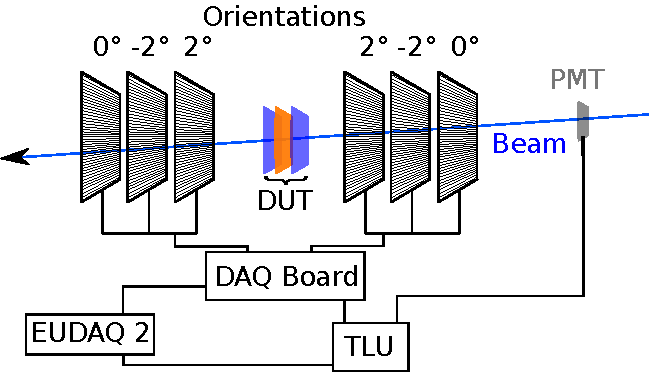
\includegraphics[width=0.49\linewidth]{pics/principle.pdf}
%}%
%\hspace{150px}
%\begin{minipage}{1.2in}%
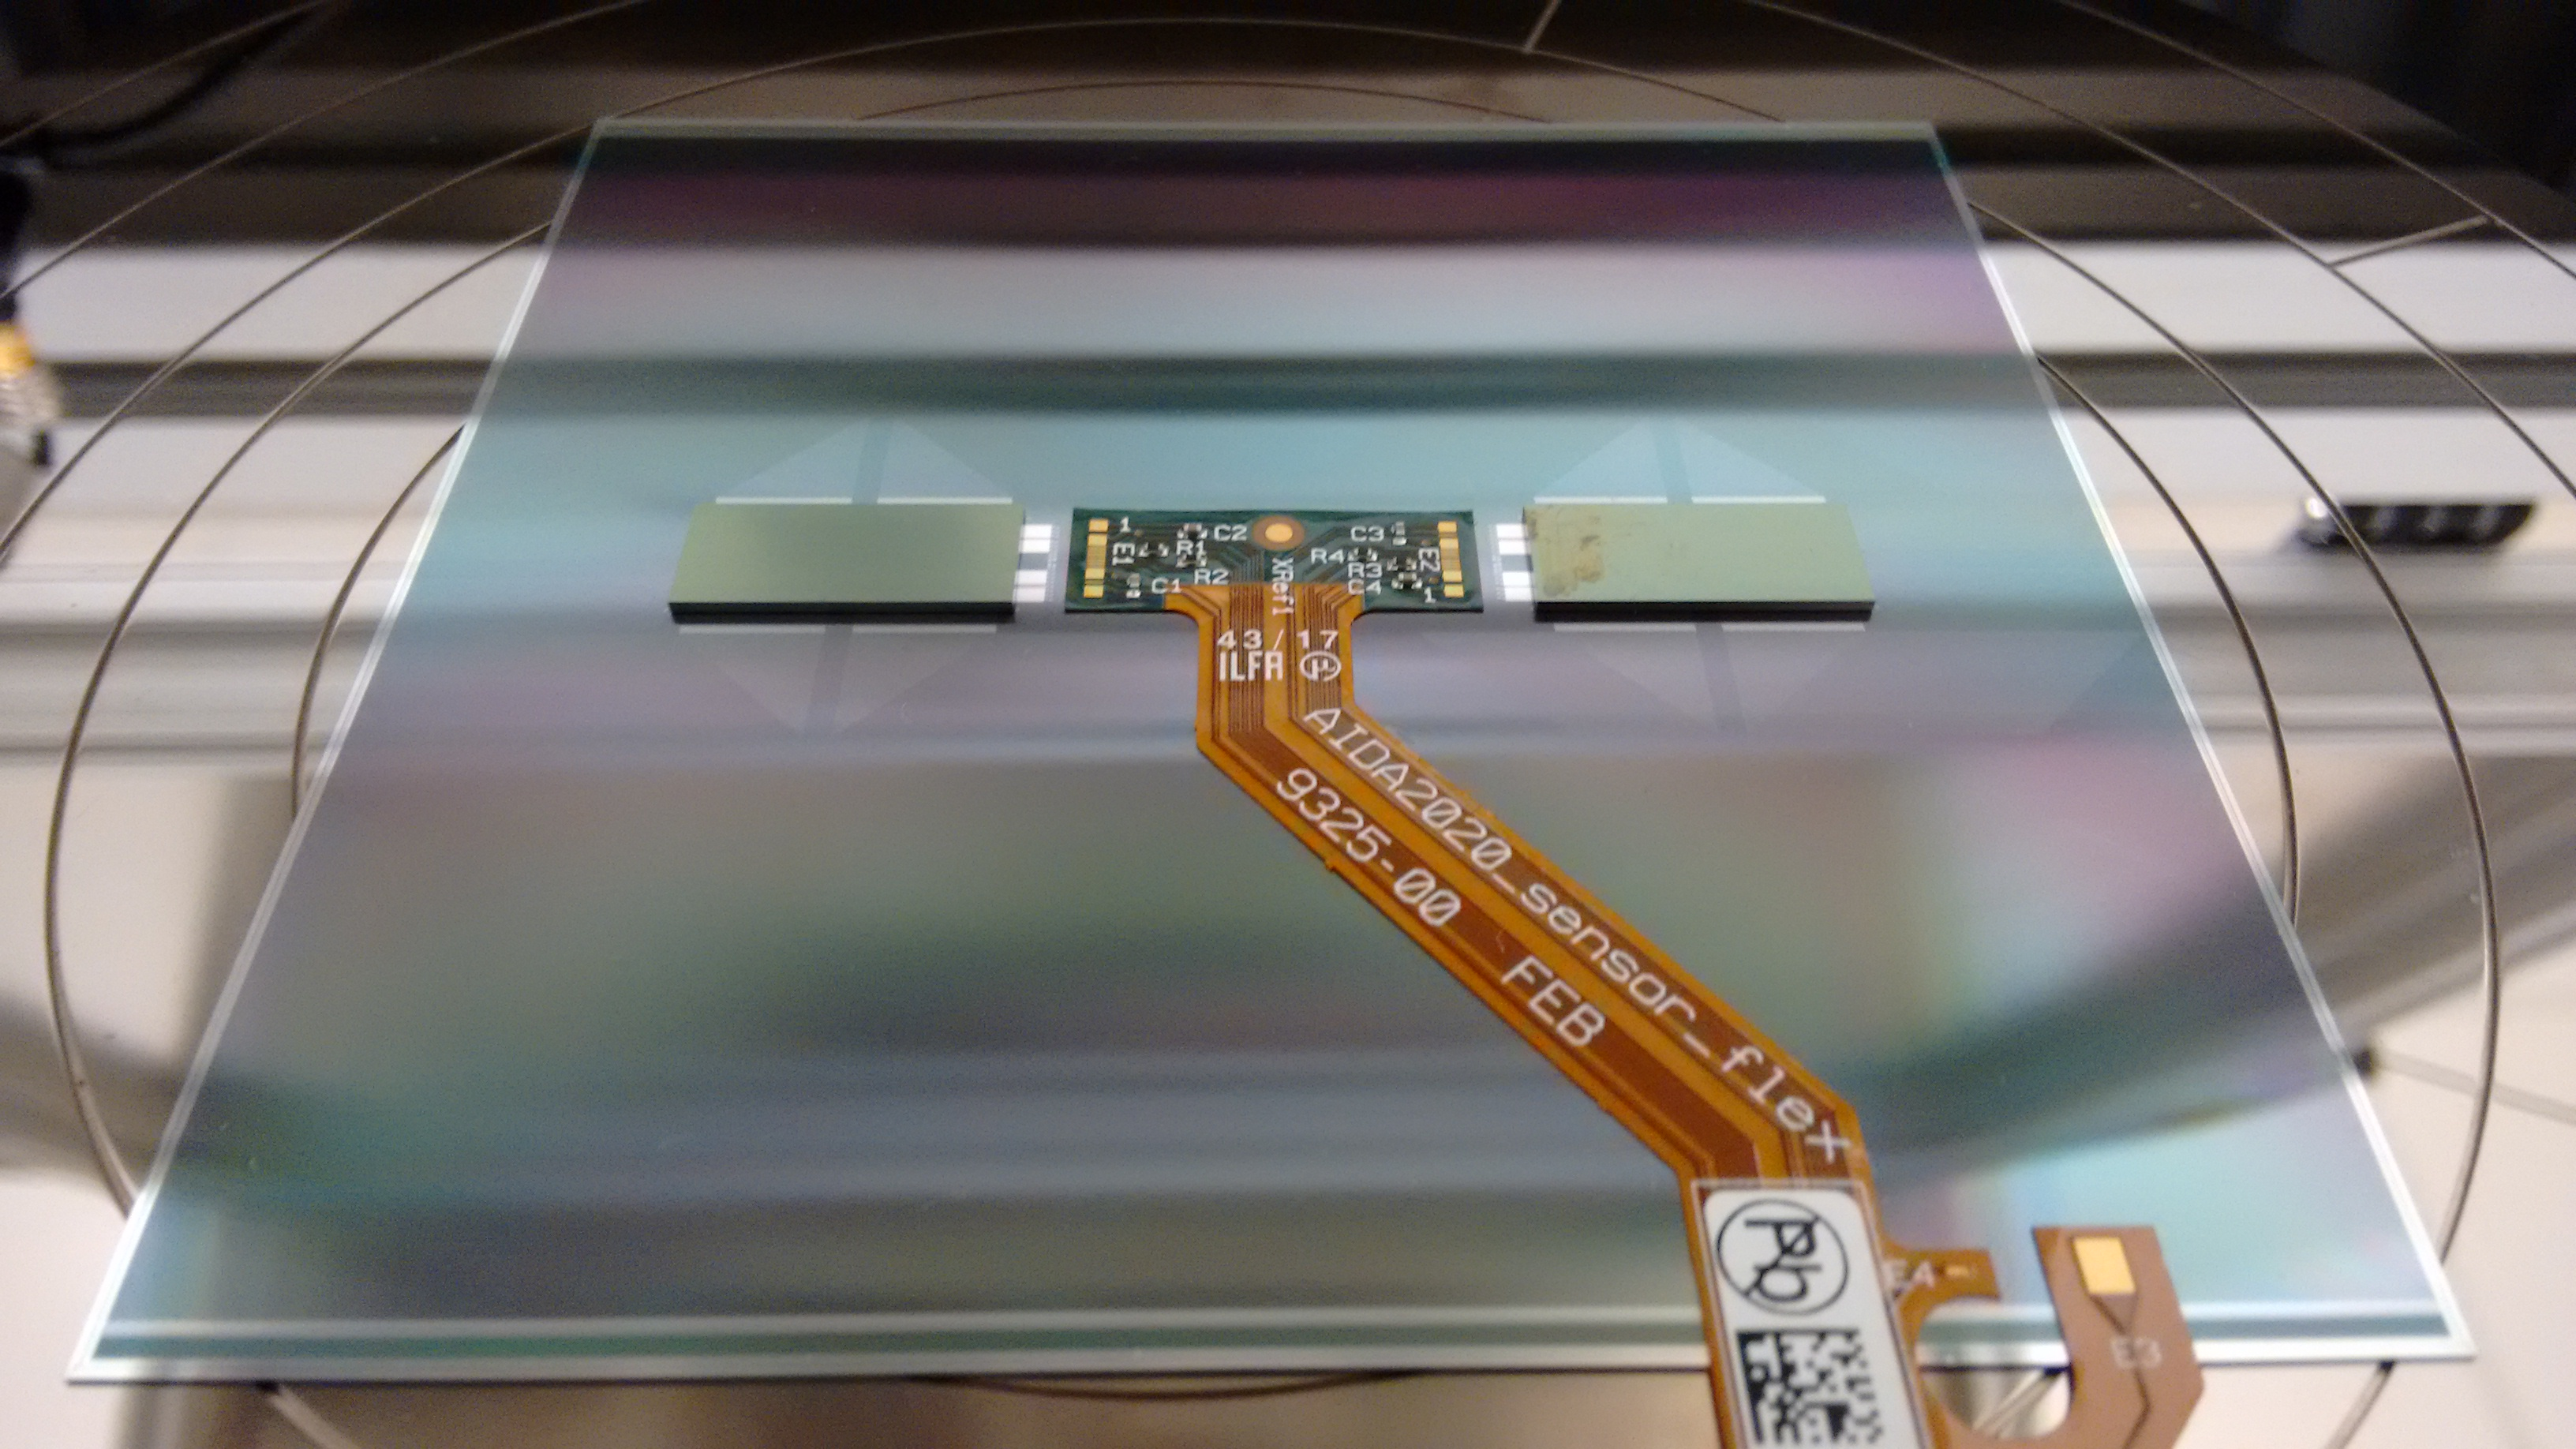
\includegraphics[width=0.49\linewidth]{pics/sensor_module1.jpg}
%\end{minipage}%
\caption{Left: sketch of the \lycoris telescope, where the black lines show the connections of modules;
Right: photo of one assembled module with 2 bumpbonded KPiX chips connecting to a kapton cable glued on sensor via wirebonding.}%
\label{fig:1figs}%
\end{figure}

The 10$\times$\SI{10}{\square\centi\metre} SiD tracker strip sensor at a pitch of \SI{25}{\micro\metre}, readout by 2 1024-channel ASICs, KPiX~$^{\cite{kpix}}$, can provide a resolution of around \SI{7.2}{\micro\metre},
was hence chosen, and the other requirements can be achieved by a \SI{2}{\degree} tilt.
The new telescope, \lycoris is finally designed as a 6-plane strip telescope in a mirror symmetric setup, with its upperstream orientation of (0, -\SI{2}{\degree}, \SI{2}{\degree}), see Figure~\ref{fig:1figs} (left), and it is controlled by a data acquisition (DAQ) FPGA board.
When a beam particle passes a Photomultiplier (PMT), the connected Trigger Logic Unit (TLU) will send a trigger to the telescope and to the DUT for synchronization;
the telescope data is digitized and readout by the bumpbonded KPiXs, then packed by the DAQ board and sent to the connected PC, the total integration time is .
A common DAQ software from the beam telescope community, EUDAQ2~$^{\cite{eudaq2}}$, is used, which also helps to synchronize the run control of telescope, TLU, and DUT.

\section*{Assembly and Tests}

The KPiX readout system were characterized before the sensor delivery with some known hexagonal pixel sensors,
including understanding how to synchronize the KPiX chip data taking cycles to the DESY beam structure, as well as to other devices, like TLU, and various DUTs.
It was tested first with a Sr90 source in the lab, and then in the DESY test beam with energies from 4 to \SI{6}{\GeV} in May and October 2017~\cite{lycoris1}.

The strip sensors were delivered by Hamamtsu in summer 2017, showing very good electric features and all fully depleted at around \SI{50}{\volt}.
The first assembled sensors, see one example in Figure~\ref{fig:1figs} (right), were tested in spring 2018, with a Sr90 source in the lab at DESY, and several DESY test beam weeks are in schedule in fall 2018.
Figure~\ref{fig:2figs} shows the fired strip distribution over one data taking run, collected by one KPiX chip from one assembled module, under a Sr90 source in a self-trigger mode,
demenstrating that the assembled module is capable of seeing signals.

\begin{figure}[!ht]%
\centering
%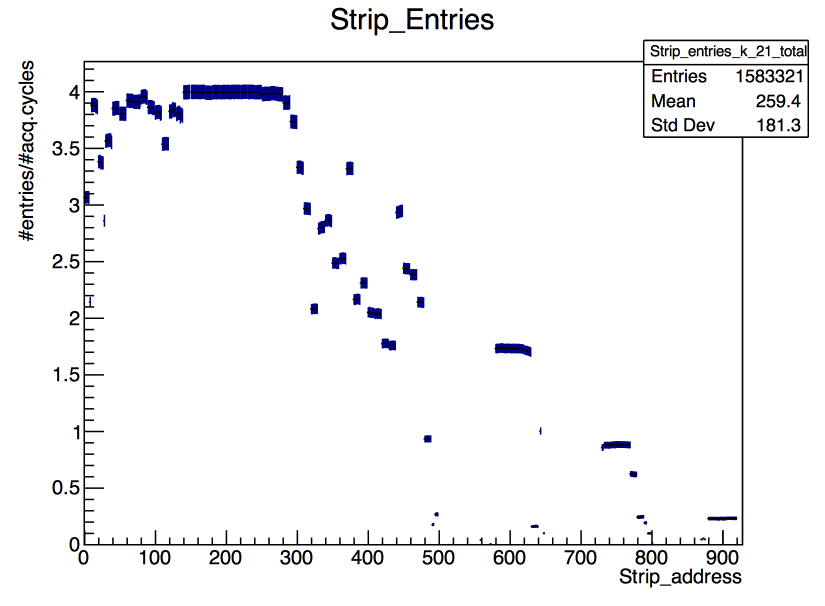
\includegraphics[width=0.49\linewidth]{pics/S58_K2_2018_05_07_16_49_42_strip_entries.png}
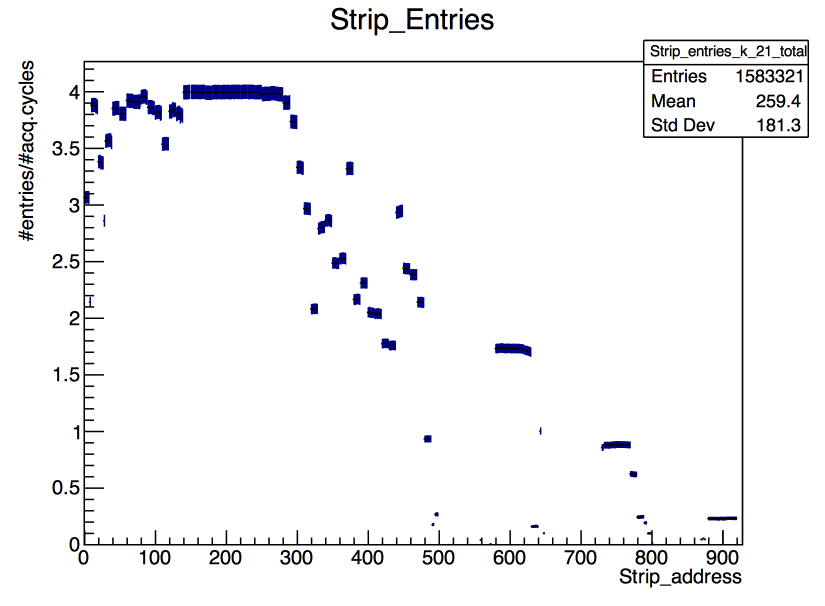
\includegraphics[width=0.49\linewidth]{pics/S58_K2_2018_05_07_16_49_42_strip_entries.png}
\caption{The fired strip distribution over one assembled module, data collected from one KPiX in a self-trigger mode under a Sr90 source. }%
\label{fig:2figs}%
\end{figure}

\lycoris telescope is scheduled to be delivered early 2019, with a TLU and a reconstruction software ready-to-use for user.
In this contribution, the latest \lycoris prototype will be presented, with its first results and a comparison to simulation;
the characterization of the sensor and readout system will also be included.

\footnotesize
\begin{thebibliography}{1}

\bibitem{eudet} H.~Jansen et al., {\em Performance of the EUDET-type beam telescopes},
\textbf{EPJ Tech.\ Instrum.\  {\bf 3}, no. 1, 7 (2016)}.

\bibitem{kpix} J.~Brau et al., {\em KPiX - A 1,024 channel readout ASIC for the ILC},
\textbf{in 2012 IEEE Nuclear Science Symposium and Medical Imaging Conference Record (NSS/MIC), pp. 1857–1860, Oct 2012.}.

\bibitem{eudaq2} Y.~Liu., {\em EUDAQ2 User Manual},
\textbf{AIDA-2020-NOTE-2018-001}.

\bibitem{lycoris1} U.~Kraemer et al., {\em LYCORIS - A Large Area Strip Telescope},
\textbf{arXiv:1801.08505 [physics.ins-det]}.

%\bibitem{T3B} The CALICE Collaboration, C. Adloff et al., {\em The time structure of hadronic showers in highly granular calorimetres with tungsten and
%steel absorbers}, \textbf{2014 JINST 9 P07022}.

\end{thebibliography}

\end{document}
